%%% template.tex
%%%
%%% This LaTeX source document can be used as the basis for your technical
%%% paper or abstract. Intentionally stripped of annotation, the parameters
%%% and commands should be adjusted for your particular paper - title, 
%%% author, article DOI, etc.
%%% The accompanying ``template.annotated.tex'' provides copious annotation
%%% for the commands and parameters found in the source document. (The code
%%% is identical in ``template.tex'' and ``template.annotated.tex.'')

%\documentclass[annual]{acmsiggraph}
\documentclass[review]{acmsiggraph}            

\usepackage{subfigure}



%% The 'graphicx' package allows for the inclusion of EPS figures.

\usepackage{graphicx}

%% use this for zero \parindent and non-zero \parskip, intelligently.

\usepackage{parskip}

%% Optional: the 'caption' package provides a nicer-looking replacement
%% for the standard caption environment. With 'labelfont=bf,'textfont=it',
%% caption labels are bold and caption text is italic.

\usepackage[labelfont=bf,textfont=it]{caption}

%% If you are submitting a paper to the annual conference, please replace
%% the value ``0'' below with the numeric value of your OnlineID.
%% If you are not submitting this paper to the annual conference,
%% you may safely leave it at ``0'' -- it will not be included in the output.

\usepackage{color}

\graphicspath{{images/}}

%% paper: 1046
\TOGonlineid{1046}
\TOGvolume{0}
\TOGnumber{0}
\TOGarticleDOI{1111111.2222222}
\TOGprojectURL{}
\TOGvideoURL{}
\TOGdataURL{}
\TOGcodeURL{}

\title{Project PAALM: Phalangeal Angle Approximation through the Leap Motion Controller}

\author{Michael L. Rivera\thanks{e-mail:mrivera.lee@gmail.com}\\University of Pennsylvania}
\pdfauthor{Aline Normoyle}

\keywords{user interfaces,motion capture,hand animation}

\begin{document}

%% \teaser{
%%   \includegraphics[height=1.5in]{images/sampleteaser}
%%   \caption{Spring Training 2009, Peoria, AZ.}
%% }

\teaser{
\centering
\subfigure[]{
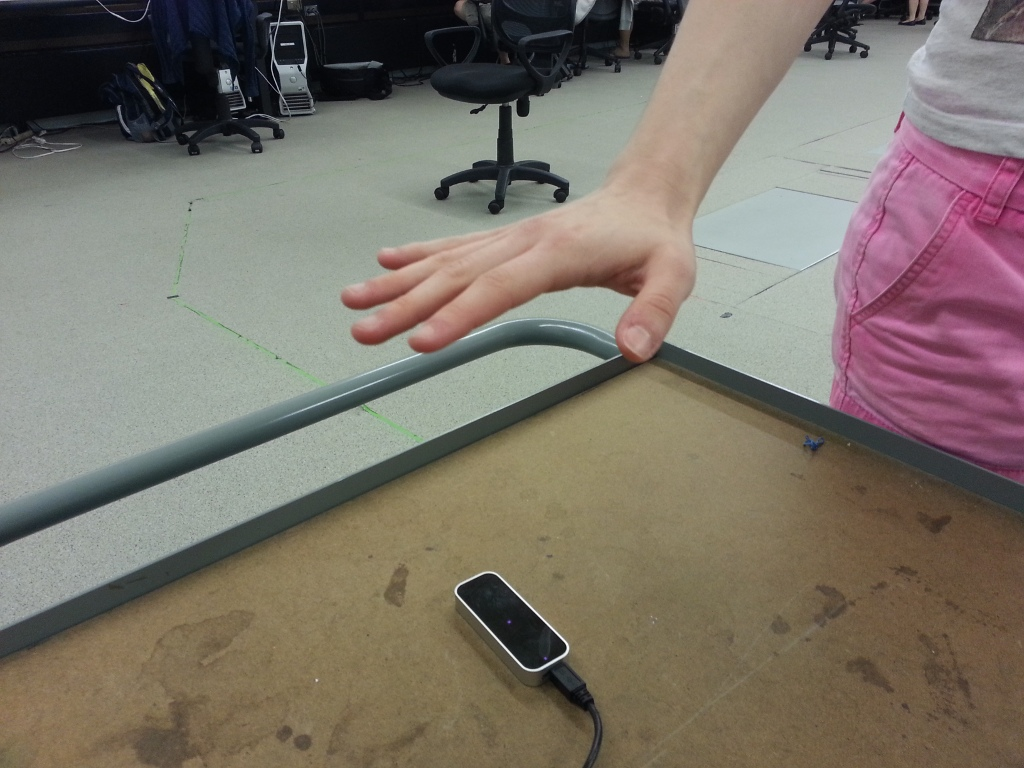
\includegraphics[scale = 0.1]{hand-input-01.jpg}
\label{fig:Video1}
}
\subfigure[]{
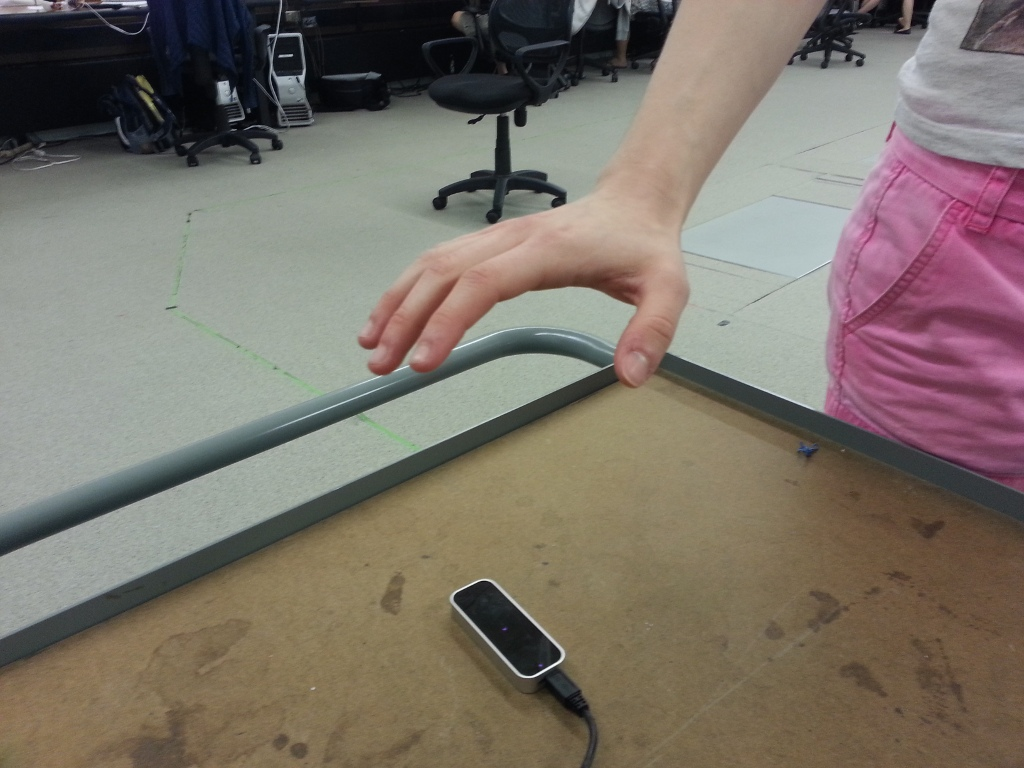
\includegraphics[scale = 0.1]{hand-input-02.jpg}
\label{fig:Video2}
}
\subfigure[]{
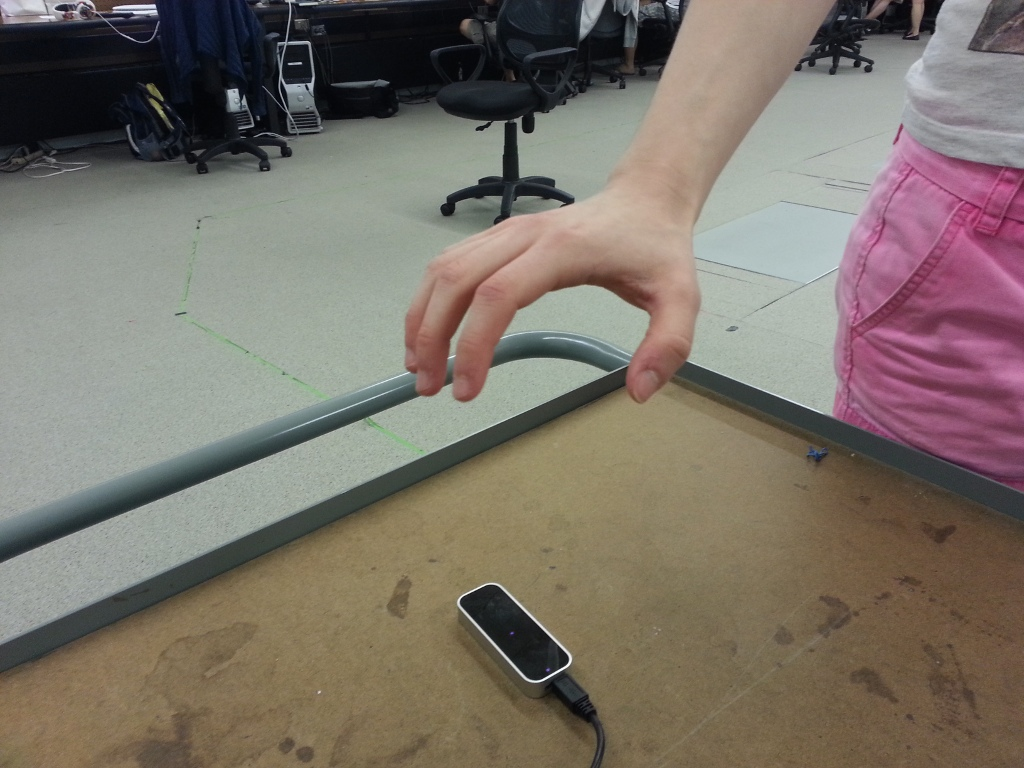
\includegraphics[scale = 0.1]{hand-input-03.jpg}
\label{fig:Video3}
}
\subfigure[]{
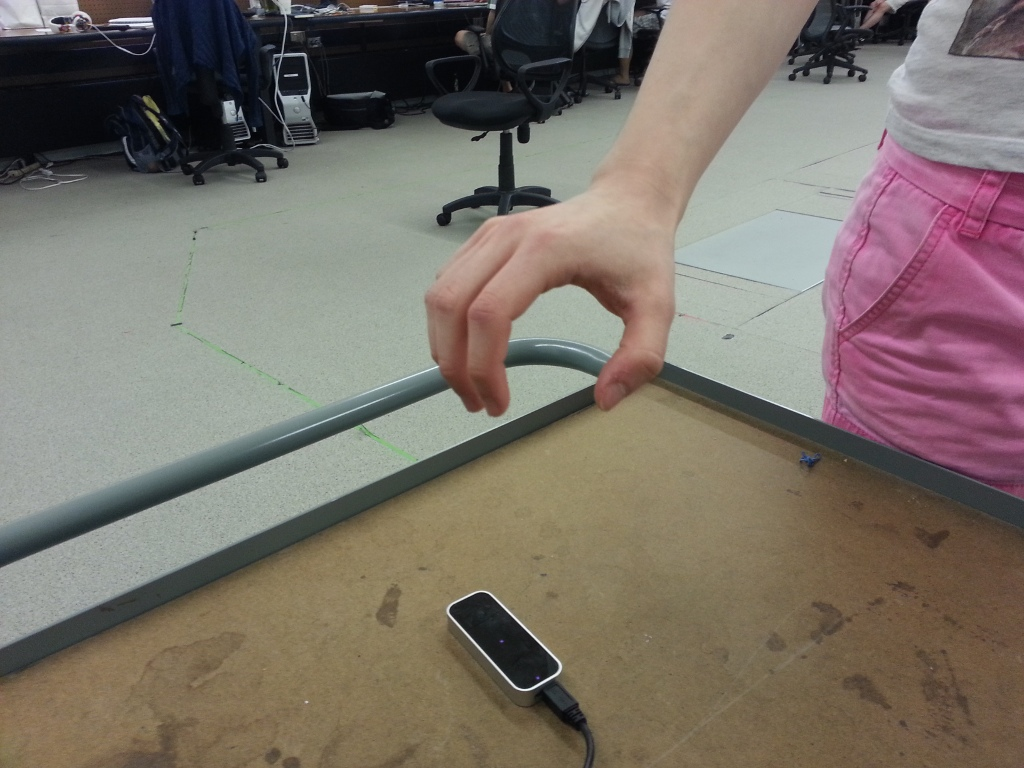
\includegraphics[scale = 0.1]{hand-input-04.jpg}
\label{fig:Video4}
}
\subfigure[]{
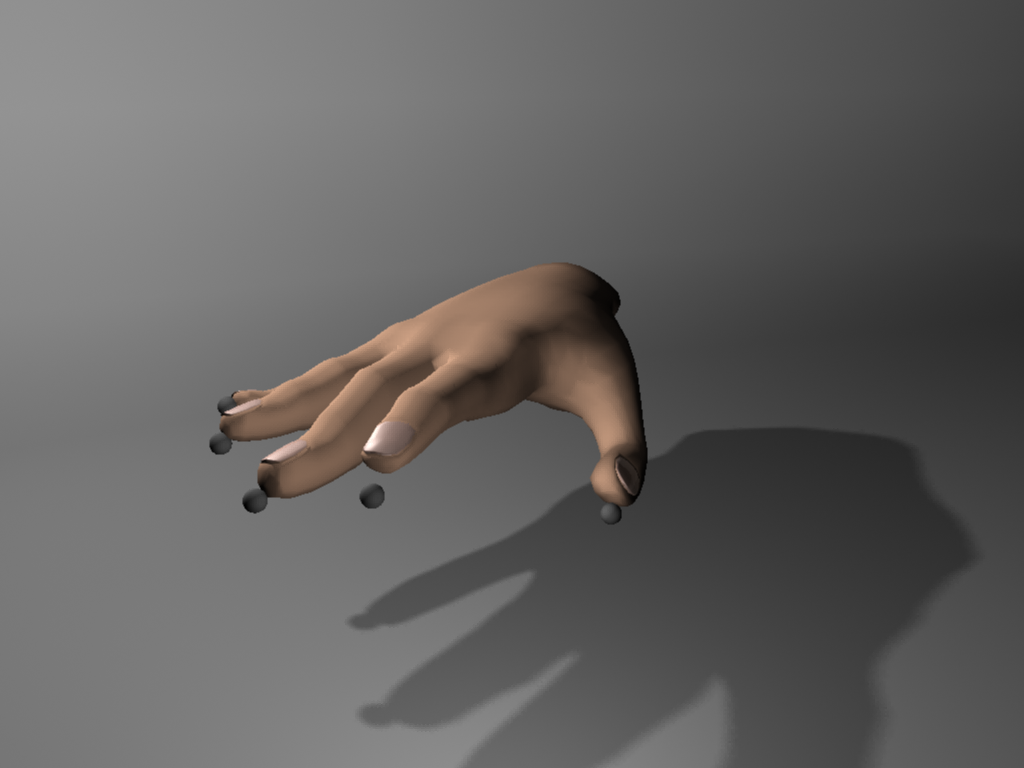
\includegraphics[scale = 0.1]{hand-rendered-01.png}
\label{fig:Maya1}
}
\subfigure[]{
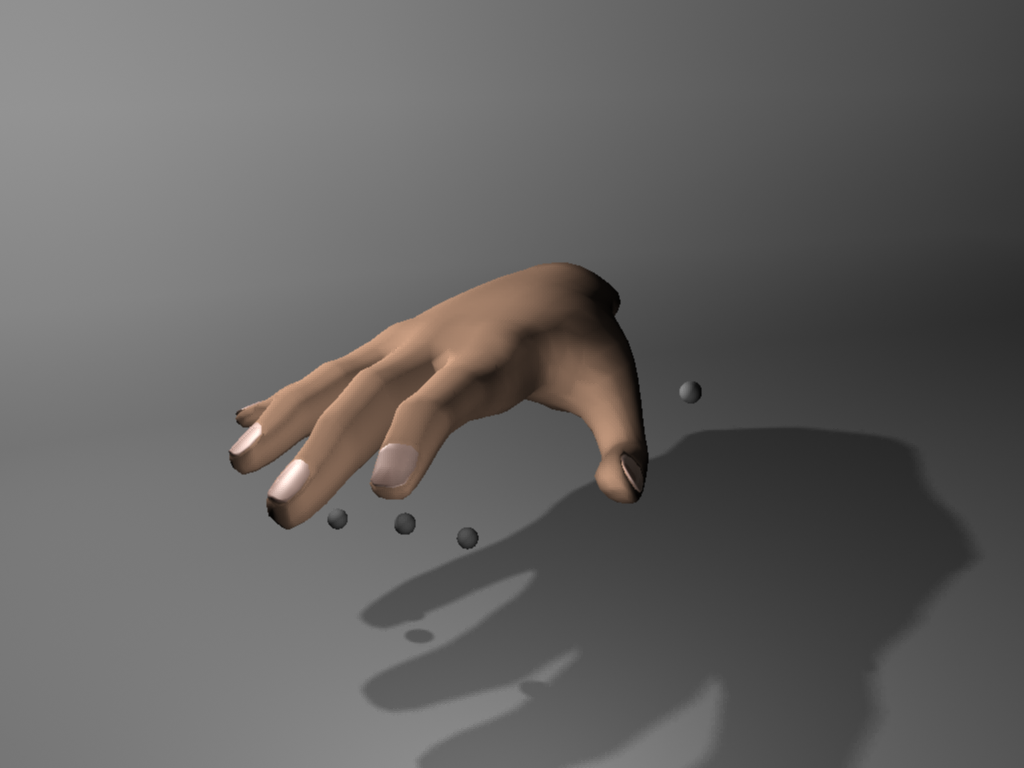
\includegraphics[scale = 0.1]{hand-rendered-02.png}
\label{fig:Maya2}
}
\subfigure[]{
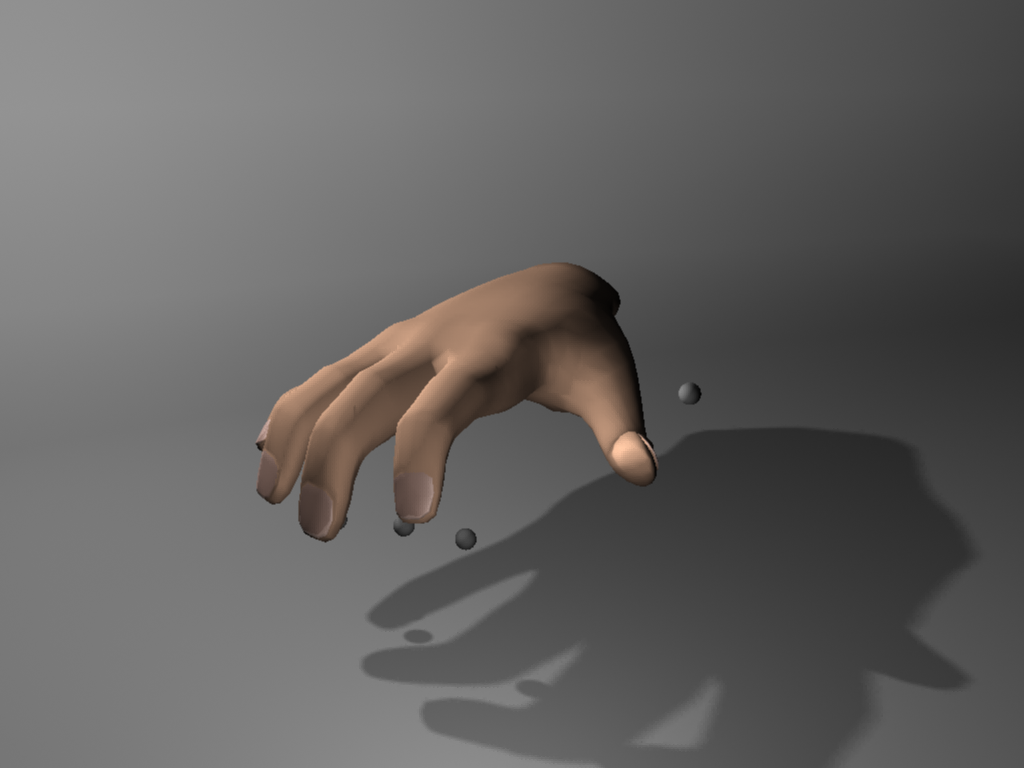
\includegraphics[scale = 0.1]{hand-rendered-03.png}
\label{fig:Maya3}
}
\subfigure[]{
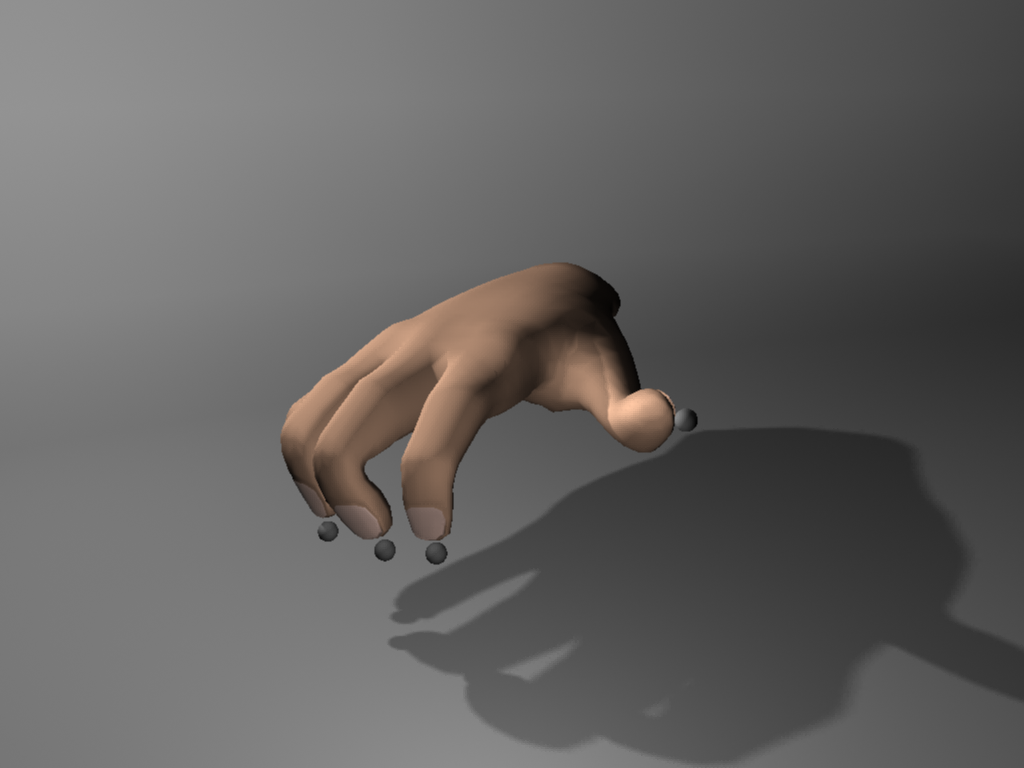
\includegraphics[scale = 0.1]{hand-rendered-04.png}
\label{fig:Maya4}
}
\vspace{-0.3cm}
\caption{Top Left to Right: The Leap Motion controller tracks to palm and fingers above it. 
Bottom Left to Right: Our PAALM system estimates finger positions in real-time based on the Leap input. 
The bottom animation was created using a Maya plugin which communicates directly with the device to 
create keyframes for a hand model which correspond to the live input.}
\vspace{-0.5cm}
}



\maketitle

\begin{abstract}

A significant problem in computer graphics has been the
realistic animation of the human hand. The dexterity and
flexibility of the hand make it difficult to accurately capture
information about complex gestures. Current approaches
are expensive, restrict movement of the hand, confine the
user to a capture region, or cannot capture hand motion
data in real time.
We propose an accurate and inexpensive method for approximating
phalangeal joint angles of the hand using the
Leap Motion Controller. Our method provides an application
programming interface for the approximation and
visualization of the phalangeal joint angle data for use with
the Leap Motion Controller.

\end{abstract}

% TODO
\begin{CRcatlist}
  \CRcat{I.3.3}{Computer Graphics}{Three-Dimensional Graphics and Realism}{}
  \CRcat{I.3.7}{Computer Graphics}{Three-Dimensional Graphics and Realism}{};
\end{CRcatlist}

\keywordlist

\TOGlinkslist

\copyrightspace

\section{Introduction}

Our hands are very dexterous and versatile. They are the
principal mechanism we use to interface with the physical
world. In computer graphics, the realistic animation of the
human hand has been a fundamental problem ~\cite{ZCX12}.
Detailed and subtle finger motions and hand movements
help bring characters to life but are often difficult to capture.
A great deal of research has been devoted to better
describing the hand and its complexities. Imaged-based,
glove-based, and marker-based techniques have been developed
to obtain descriptive data regarding hands movements
and gestures. These methods, however, are expensive,
restrict the motion of the hand, confine the user to a
space, or cannot be accomplished in real time.
We propose an effective method for approximating phalangeal
joint angles of the hand that is portable, unrestrictive
and cost-effective. Our approach utilizes a new and
unexplored technology called the Leap Motion Controller
that is roughly the size of a flash drive and tracks individual
finger movements to 1/100th of a millimeter ~\cite{LEA}. Our
approach implements an application programming interface
for approximating and visualizing the phalangeal joint
angles of the hand.

Contributions.
Our main contributions are as follows:
• An accurate, portable, cost-effective, and freehand
method of obtaining phalangeal joint angles using an
unexplored technology.
• An application programming interface (API) for obtaining
and visualizing the phalangeal joint angle data
using the Leap Motion Controller.

The target audience of this project is the computer
graphics and animation industry. We aim to provide an
effective approach to approximating phalangeal joint angles
of the hand. Our approach differs from current offerings
because it is unrestrictive, requiring no sensors to be
attached to the hand, and is inexpensive. While our main
focus is in the computer graphics and animation industry,
we do not discount the applicability of our approach to
additional fields. The detection of phalangeal joint angles is
useful in many other fields such as Human Computer Interaction
(HCI) for the development of Natural User Interfaces
(NUI), and robotics for the simulation of human gestures
through mechanical means.

Our method will achieve the following functionality:
- Approximate phalangeal joint angles using the Leap
Motion Controller.
- Visualize the approximated phalangeal joint angle
data.

\section{Related Work}

The problem of hand motion recognition is ubiquitous
making it a considerable research focus for many fields like
computer graphics. A number of systems have been developed
to detect and obtain descriptive data about hand gestures.

\subsection{Marker-based Systems}

Marker-based motion capture systems are a popular
means of obtaining hand motion data. The standard approach
requires attaching approximately 30 retro-reflective
markers to the hand and tracking them over time ~\cite{VIC}.
The temporal data is then used to reconstruct a 3D representation
of the hand and its motions.
Recent advancements in hand motion capture have made
it possible to achieve descriptive hand motion data with a
reduction in the number of markers ~\cite{HRM12}. Though
even with such advancements, marker-based approaches
still pose significant problems in hand motion detection.
Gestures featuring self-occlusion (fingers overlapping one
another) are difficult to detect using the system. Automatic
marker tracking is not effective in maintaining the markers
over time. Thus, the process of tracking markers is then a
tedious one, requiring manual labeling that is both time consuming
and error prone ~\cite{ZCX12}.


\subsection{Glove-based Systems}

Glove-based systems such as the CyberGlove ~\cite{CYB}
provide a useful method of obtaining hand gesture data that
is free from issues that arise when fingers occlude each
other. The motions recorded using the system, however, are
often noisy and fail to capture delicate articulations with
high precision ~\cite{ZCX12}. Likewise, the system restricts the
natural motion of the hand, making capturing realistic gestures
a more complex task. The advantage of using the
Leap Motion Controller for our approach is that it permits
the hand to move freely and naturally.


\subsection{Image-based Systems}

Computer vision has offered a promising alternative to
data gloves and other worn mechanisms for detecting hand
motions ~\cite{EBN07}. Image-based systems have allowed for
some natural hand movements to be detected and offer a
less expensive approach to marker-based systems. Typically,
the process analyzes a series of image frames to reconstruct
the gesture of a hand and project it to a hand model
through inverse kinematics.
A recent device called Digits has been developed that
uses a wrist-worn gloveless sensor to detect 3D hand gestures
~\cite{KHI12}. The sensor features two infrared illumination
schemes that are used to produce a hand model
through inverse kinematics. The wrist-worn device avoids
the need for any embedded sensors in the environment and
permits the hand to move freely as well as the user to move
about without being confined to a capturing region.
Computer vision techniques do have limitations in obtaining
hand motion data. The process is computationally
intensive. Systems using inverse kinematics for the fingers
and the rotation of the palm are solved by numerical iteration
[LK93]. Better results are obtained by running numerous
iterations. Some processes also pose limitations by
only providing support for a small range of hand actions
under restrictive conditions. Thus real time detection can
only be accomplished if there already exists a vocabulary
of recognized gestures. Additionally, computer vision techniques
do not fair well under conditions that create self occlusion,
namely fingers overlapping or blocking the view
of each other with respect to the camera.

\subsection{Joint Systems}

A recent innovation has been combining marker-based
and image-based systems to provide higher fidelity hand
motion data ~\cite{ZCX12}. These systems are capable of accurately
detecting hand motions even in cases of self occlusion.
The markers are used as reference when rebuilding
hand motion data using an RGB-depth camera such as
the Microsoft Kinect. These systems are robust and do not
significantly restrict hand movements as the markers are
small. The shortcoming of this system is that it currently
cannot produce results in real time and requires a user to be
confined to a particular space.

\section{LEAP}



The Leap Motion Controller offers a cost-effective, fast
and precise means of capturing live hand motion data. In
addition, the small size of the device makes it easily portable.
In our implementation, we leverage these features to
provide real time data about articulated phalangeal joint
angles on the hand.


\begin{figure}
\centering
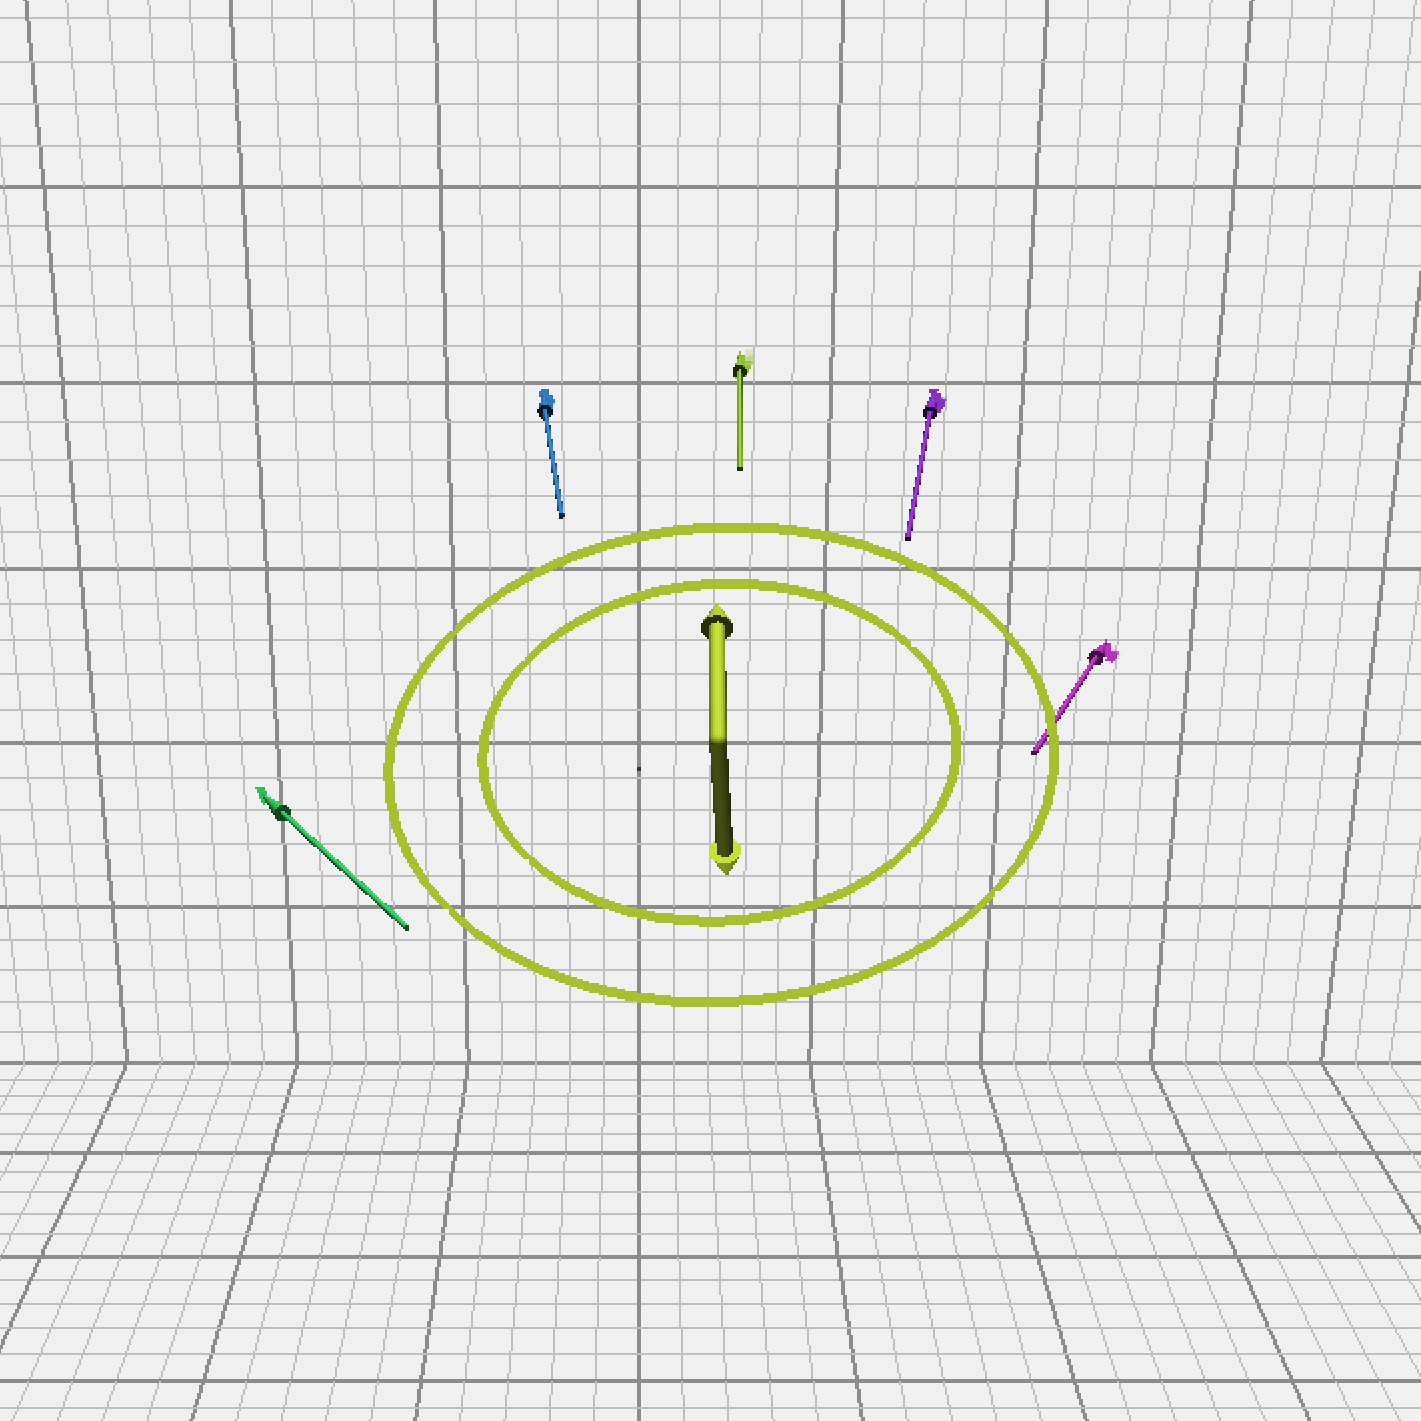
\includegraphics[scale=0.27]{leap-palm-and-fingers.png}
\vspace{-0.1cm}
\caption{Leap Motion visualizer displaying finger vectors and a palm normal for a hand. \label{HighLevel}}
\vspace{-0.5cm}
\end{figure}



\begin{figure}
\centering
\subfigure[]{
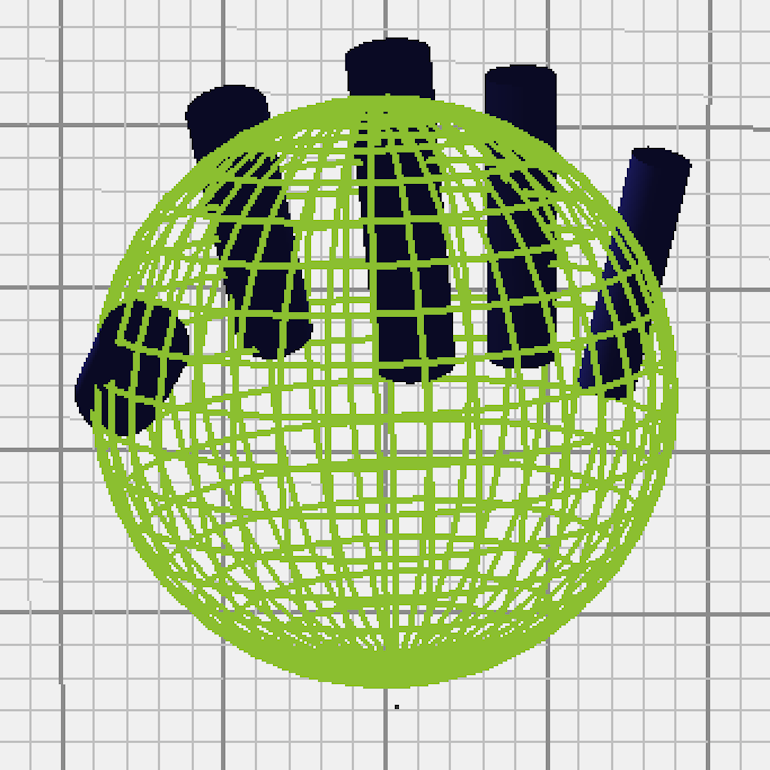
\includegraphics[scale=0.25]{palm_small_radius.png}
\label{fig:Palm1}
}
\subfigure[]{
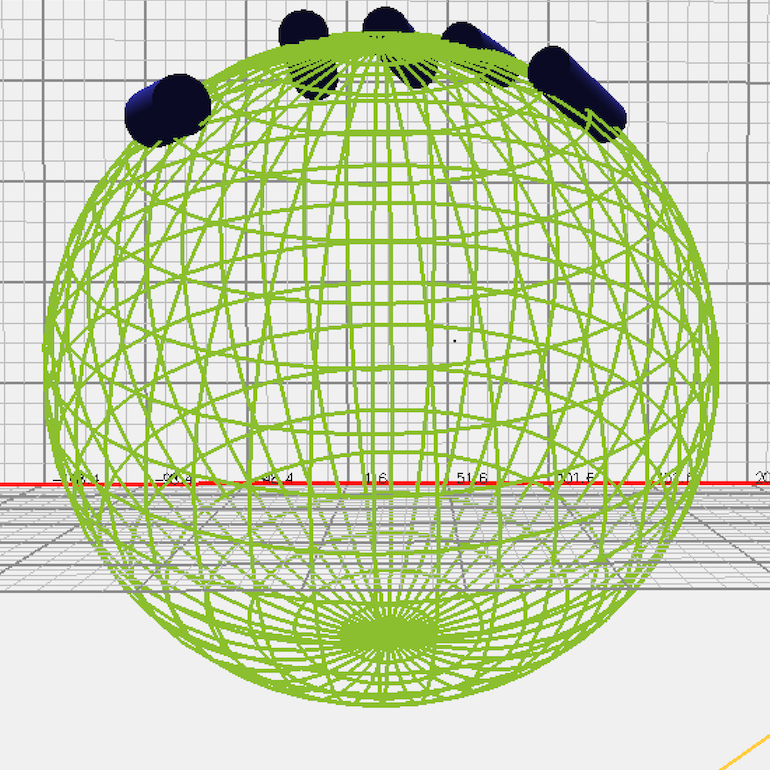
\includegraphics[scale=0.25]{palm_large_radius.png}
\label{fig:Palm1}
}
\vspace{-0.1cm}
\caption{Top to Bottom: Leap Motion visualizer displaying the palm radius for a partially closed hand and an open hand with spread fingers.\label{HighLevel}}
\vspace{-0.5cm}
\end{figure}


Background about the LEAP controller ~\cite{LEA}.[Need LEAP citation]: How does it work? What data 
do you get from it?  Include screenshots form the dev toolkit.

The Leap Motion Controller is an infrared-based device, featuring three infrared LEDs and two light sensors. The device is capable of tracking position changes as small as a 1/100th of a millimeter within a detection region of eight cubic feet. Its sensors capture spatial information at 290 frames per second and provide data about the tip position, tip velocity, length, direction, and width of pointable objects, such as a pen or a finger, in 3D space. 

With respect to fingers, the device can determine to which hand a set of fingers belong and provide details about a hand's palm position and normal. Additionally, the hand data includes a palm sphere radius, or the radius of a spherical object that could be held within the palm of the hand. A small radius suggests a closed hand while a large radius suggests an open hand with fingers spread further apart.  

All of the data provided by the Leap Motion Controller is organized into an individual frames which can be accessed and manipulated using the device's application programming interface.

The Leap Motion Controller is not currently available to the general public. We were able to obtain a developer release of the controller through an application process available on the Leap Motion web site.  An official release date for the device has been set for May 13, 2013. The cost of the device will be  \$79.99. 



\section{Approach}

\begin{figure}
\centering
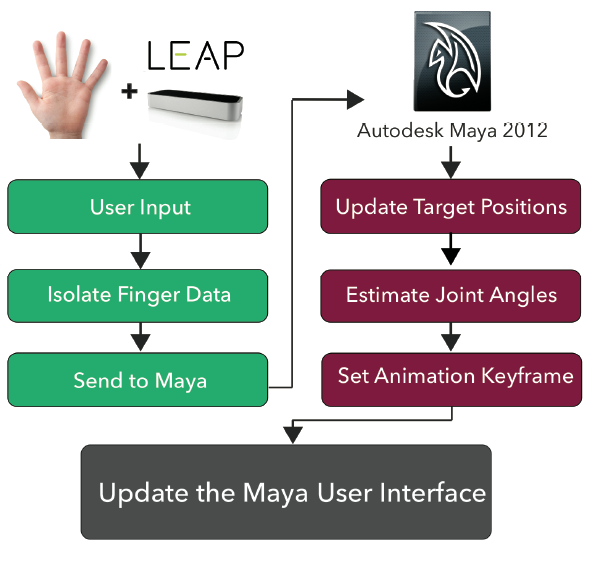
\includegraphics[scale=0.4]{Overview.png}
\vspace{-0.8cm}
\caption{PAALM Overview\label{HighLevel}}
\vspace{0.20cm}
\end{figure}


We investigate two simple methods for approximating hand positions from 
input LEAP device.

The first computes targets for each finger based on the LEAP input and 
uses IK for each finger to track the target. 

The second maps keyframes to input finger ratios and blends based on 
the ratios

Our approach has two main components: a Python script for interfacing with the Leap Motion Controller and a Maya plug-in written in PyMel for animating hand motions.

We first obtain finger data using the Leap Motion API. We recognize that hands and fingers come in a multitude of shapes and sizes. To account for individual differences, we perform an initialization process using a rest hand pose that features an open palm and spread fingers. We average the length of each individual finger of the hand over a series of one thousand frames. The average length of each finger becomes a standard for comparison in all subsequently captured frames. 

The finger data for a hand received from the Leap Motion Controller is not guaranteed to be ordered. To ensure the finger lengths we are interpreting match the fingers we expect, we sort the finger data by x-coordinates in 3D space. The x-axis is favorable because it matches the orientation of a detected hand in the device's coordinate space. We use the right hand in our system. Though the system is suitable for either hand. The sorted fingers receive unique identifiers that are used to associate standard lengths with lengths from subsequent frame updates. 

We interpret subsequent frame updates by obtaining the current finger length and the direction vector of each finger detected. The current length of a finger is useful because its detection signifies a change in the joint angles of the finger. A smaller length with respect to the standard length implies that the angles have bent in manner that brings end effector closer to the base of the finger. We leverage this aspect to achieve an approximation of joint angles. We compute a length ratio for each finger by dividing the finger's current length by its associated standard length. The direction vector, length ratio, and identifier of each finger are then sent to the Maya plug-in.

Communication with the Maya plug-in is socket-based, occurring through Maya's command port. The plug-in features a script that receives all of the direction, length ratio, and identifier data for each Leap-detected finger. The identifiers associate the direction and length ratio for each Leap-detected finger with a chain of joints in Maya. We designate each joint chain as a Maya-finger. 

Each Maya-finger is initialized with a length based on the joint positions in the finger's joint chain. The length is obtained through the summation of the vector magnitudes between a joint and its succeeding joint for every joint in a Maya-finger. The Maya-finger is assigned a target sphere that designates a point in 3D space for use with inverse kinematics. 

The Maya plug-in processes the finger data by selecting a Maya-finger that corresponds to a unique identifier provided by a Leap-finger. The correspondence between two fingers permits us to map input user hand motions to target positions in Maya. For each Leap-finger, we normalize the direction vector and multiply it by the length ratio. The product is a direction vector with a length scaled to approximate the bend of the fingers detected by the Leap. We multiply the scaled direction vector by the length of the Maya-finger to map this direction vector to the Maya coordinate space with respect to the Maya-finger. 

A new target position for the Maya-finger is computed by adding the scaled direction vector to the base position of the Maya-finger. The base position is designated by the first joint in the Maya-finger's joint chain. We use the position of the knuckle joint for each finger as the base position. We set the position of the target sphere to be this new target position and perform IK to approximate new joint angles for the Maya-finger. Upon completion IK, we set an animation keyframe so to achieve a playback animation from the input hand gestures.




LIMITATIONS


%\begin{equation}
% \sum_{j=1}^{z} j = \frac{z(z+1)}{2}
%\end{equation}
%
%\begin{eqnarray}
%x & \ll & y_{1} + \cdots + y_{n} \\
%  & \leq & z
%\end{eqnarray}


\section{Results}

Plug-in Description:
Easily applicable to other bodily appendages for animation for characters. CCD can be swapped out for a more optimized approach - database of gestures (and mapping)
Though only the human hand was demonstrated, the Maya plug-in interface permits the use of Maya-fingers with an arbitrary number of joints. The Leap finger data can easily be applied to applied to non-human appendages such as tentacles or spider legs. 

\section{Conclusion}


%\section*{Acknowledgements}

\bibliographystyle{acmsiggraph}
\bibliography{riverapalm}
\end{document}
